\section{Le jeu de rôle, un conte interactif}

\begin{shadequote}
L'art de raconter des histoires est toujours l'art de reprendre celles que l'on a entendues. \par\emph{Walter Benjamin, Der Erzähler}
\end{shadequote}

%\begin{figure}[h!]
%    \centering
%    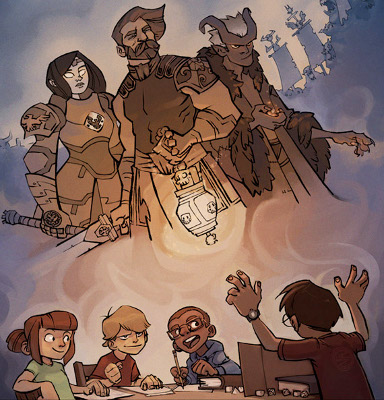
\includegraphics[width=0.80\linewidth]{img/rpg_tabletop2.jpg}
%    \caption{Tabletop RPG}
%\end{figure}

Différence entre conte et jeu de role : \\
- Personnages joueurs interagissant dans une histoire que le maître du jeu déroule pour eux, celui-ci s'adaptant à ses joueurs\\
- Univers souvent imaginaire\\
- Rarement porteur de morales, mais plutôt d'aventures\\


Similitudes :\\
- Aspect social\\
- Histoire racontée à l'oral\\
- Conteur et Maître du jeu : transporter son auditoire dans l'imaginaire\\
- Rôle essentiel de l'ambiance instaurée afin de maximiser l'immersion, et éventuellement de faire passer un message, une morale\\
- Pratique des jeux de rôle associables aux récits chevaleresques contés par les troubadours\\
- Le maître du jeu adapte son scénario aux réactions de ses joueurs. Le conteur en fait de même, en fonction de celles de son public. Le conte s'étaye par ailleurs au fil des représentations, et l'analyse des réactions du public est la clé de l'amélioration d'un conte\\

Rôle psychanalytique :\\
- L'immersion dans l'histoire permet de libérer des instincts primitifs et l'analyse des auditeurs\\
- Stimule l'imagination, dévoile des émotions et permet de mieux connaître et découvrir nos difficultés pour lesquelles nous étayons peu à peu inconsciemment des solutions\\

\clearpage
